\documentclass[11pt]{article}
\usepackage[top=1cm, bottom=2cm, left=1cm, right=1cm]{geometry}
\usepackage{ctex}
\usepackage{algorithm}
\usepackage{algorithmicx}
\usepackage{algpseudocode}
\usepackage{amsthm,amsmath,amssymb}
\usepackage[colorlinks=true,linkcolor=blue]{hyperref}
\usepackage{listings}
\usepackage{xcolor,xparse}
\usepackage{realboxes}
\usepackage{graphics}
\usepackage{graphicx}
\usepackage{mathrsfs}
\usepackage{wrapfig}
\usepackage{subfigure}
\usepackage{pifont}
\newcommand{\To}{\textbf{To} }
\definecolor{cmdbg}{rgb}{0.9,0.9,0.9}
\lstset{%
	basicstyle=\ttfamily,
	breaklines = true,
	backgroundcolor=\color{cmdbg},
}
\DeclareDocumentCommand{\ccmd}{v}{% 参数 v 表示工作方法类似于 \verb
    \Colorbox{cmdbg}{\csname lstinline\endcsname!#1!}%
}

\makeatletter
\newenvironment{breakablealgorithm}
  {% \begin{breakablealgorithm}
   \begin{center}
     \refstepcounter{algorithm}% New algorithm
     \hrule height.8pt depth0pt \kern2pt% \@fs@pre for \@fs@ruled
     \renewcommand{\caption}[2][\relax]{% Make a new \caption
       {\raggedright\textbf{\ALG@name~\thealgorithm} ##2\par}%
       \ifx\relax##1\relax % #1 is \relax
         \addcontentsline{loa}{algorithm}{\protect\numberline{\thealgorithm}##2}%
       \else % #1 is not \relax
         \addcontentsline{loa}{algorithm}{\protect\numberline{\thealgorithm}##1}%
       \fi
       \kern2pt\hrule\kern2pt
     }
  }{% \end{breakablealgorithm}
     \kern2pt\hrule\relax% \@fs@post for \@fs@ruled
   \end{center}
  }
\makeatother

\author{谢昀城 22307110070}
\title{计算物理作业8}

\begin{document}
\maketitle




  \section{题目1}
  \subsection{题目描述}
  
  Consider the Poisson equation: 
   \[
   \nabla^2 \phi(x, y) = -\frac{\rho(x, y)}{\varepsilon_0}
   \]
   from electrostatics on a rectangular geometry with \(x \in [0, L_x]\) and \(y \in [0, L_y]\). Write a program that solves this equation using the relaxation method. Test your program with:

   (a) \(\rho(x, y) = 0\), \(\phi(0, y) = \phi(L_x, y) = \phi(x, 0) = 0\), \(\phi(x, L_y) = 1 \, \mathrm{V}\), \(L_x = 1 \, \mathrm{m}\), and \(L_y = 1.5 \, \mathrm{m}\);

   (b) \(\rho(x, y)/\varepsilon_0 = 1 \, \mathrm{V/m^2}\), \(\phi(0, y) = \phi(L_x, y) = \phi(x, 0) = \phi(x, L_y) = 0\), and \(L_x = L_y = 1 \, \mathrm{m}\).



\subsection{程序描述}
   在本程序中,我们使用jacobi算法求解方形区域上的泊松方程。程序将根据迭代前后函数值的$L_{\infty}$范数来判断是否收敛。
   \[V_{i,j}^{n+1} = \frac{1}{2+2\alpha} \left[ V_{i+1,j}^n + V_{i-1,j}^n + \alpha(V_{i,j+1}^n + V_{i,j-1}^n) + \Delta x^2 \rho_{i,j} \right], \quad n = 0, 1, 2, \ldots,\alpha = \frac{\Delta x^2}{\Delta y^2}\]

本程序源文件为solvePoisson.py,在终端进入当前目录,使用命令python -u solvePoisson.py运行本程序。运行时请保证Python第三方库Numpy,Matplotlib已安装。程序开发环境为Python3.12.3,可在Python3.8以上版本中运行。

\subsection{伪代码}
\subsubsection*{求解泊松方程 伪代码:}

\begin{breakablealgorithm}
  \caption{PoissonSolver}
  \begin{algorithmic}
    \State \textbf{Class PoissonSolver}
    \State \textbf{Attributes:} $upbound$, $downbound$, $leftbound$, $rightbound$, $rho$, $Lx$, $Ly$, $Nx$, $Ny$, $dx$, $dy$, $ap$, $u$, $X$, $Y$, $rhol$
  
    \State \textbf{Method}
    \Function{InitGrid}{}
      \State $xl \gets$ linspace($0$, $Lx$, $Nx$)
      \State $yl \gets$ linspace($0$, $Ly$, $Ny$)
      \State $u \gets$ zeros(($Nx$, $Ny$))
      \State $X, Y \gets$ meshgrid($xl$, $yl$)
      \State ApplyBoundary($u$)
    \EndFunction
  
    \Function{BoundaryPos}{}
      \State \textbf{OUTPUT:} $bu$, $bd$, $bl$, $br$ (boolean 2D arrays)
      \State $bu \gets$ zeros(($Nx$, $Ny$), dtype=bool)
      \State $bd \gets$ zeros(($Nx$, $Ny$), dtype=bool)
      \State $bl \gets$ zeros(($Nx$, $Ny$), dtype=bool)
      \State $br \gets$ zeros(($Nx$, $Ny$), dtype=bool)
      \State $bu[-1, :] \gets 1$
      \State $bd[1, :] \gets 1$
      \State $bl[:, 1] \gets 1$
      \State $br[:, -1] \gets 1$
      \State \Return $bu, bd, bl, br$
    \EndFunction
  
    \Function{ApplyBoundary}{$u$}
      \State $bu, bd, bl, br \gets$ BoundaryPos()
      \State $u[bu] \gets upbound(X[bu])$
      \State $u[bd] \gets downbound(X[bd])$
      \State $u[bl] \gets leftbound(Y[bl])$
      \State $u[br] \gets rightbound(Y[br])$
    \EndFunction
  
    \Function{UpdateU}{$u$}
      \State $self.u \gets u$
      \State ApplyBoundary($u$)
    \EndFunction
  
    \Function{JacobiStep}{}
      \State \textbf{OUTPUT:} $u$ (updated 2D array of $u$)
      \State $u \gets$ zerosLike($u$)
      \State $u[1:-1,1:-1] \gets$
      \State \quad ($u[:-2,1:-1] + u[2:,1:-1] + ap \cdot (u[1:-1,:-2] + u[1:-1,2:]) + dx^2 \cdot rhol[1:-1,1:-1]) / 2 / (1 + ap)$
      \State UpdateU($u$)
      \State \Return $u$
    \EndFunction
  
    \Function{Jacobi}{$maxIter$, $tol$}
      \State \textbf{INPUT:} $maxIter$ (integer), $tol$ (float)
      \State \textbf{OUTPUT:} $u$ (2D array solution of Poisson equation)
      \State $hisig \gets$ copy($u$)
      \For{$i \gets 0$ \To $maxIter$}
        \State JacobiStep()
        \If{max(abs($u - hisig$)) $<$ $tol \cdot dx^2$}
          \State \textbf{Print:} "Jacobi converged after $i$ iterations with relative tolerance $tol$"
          \State \textbf{Break}
        \EndIf
        \State $hisig \gets$ copy($u$)
      \State \textbf{else for}
        \State \textbf{Print:} "Jacobi did not converge after $maxIter$ iterations with relative tolerance $tol$"
      \EndFor
      \State \Return $u$
    \EndFunction
  \end{algorithmic}
  \end{breakablealgorithm}
  
  
  
  
  \subsection{输入输出实例}

  对于本程序,运行后会生成图\ref{fig:1}为"solvePoisson.png"于当前目录下,分别为两种情况的求解结果。程序运行截图如图\ref{fig:p1}所示。

  \begin{figure}[ht]
    \centering
    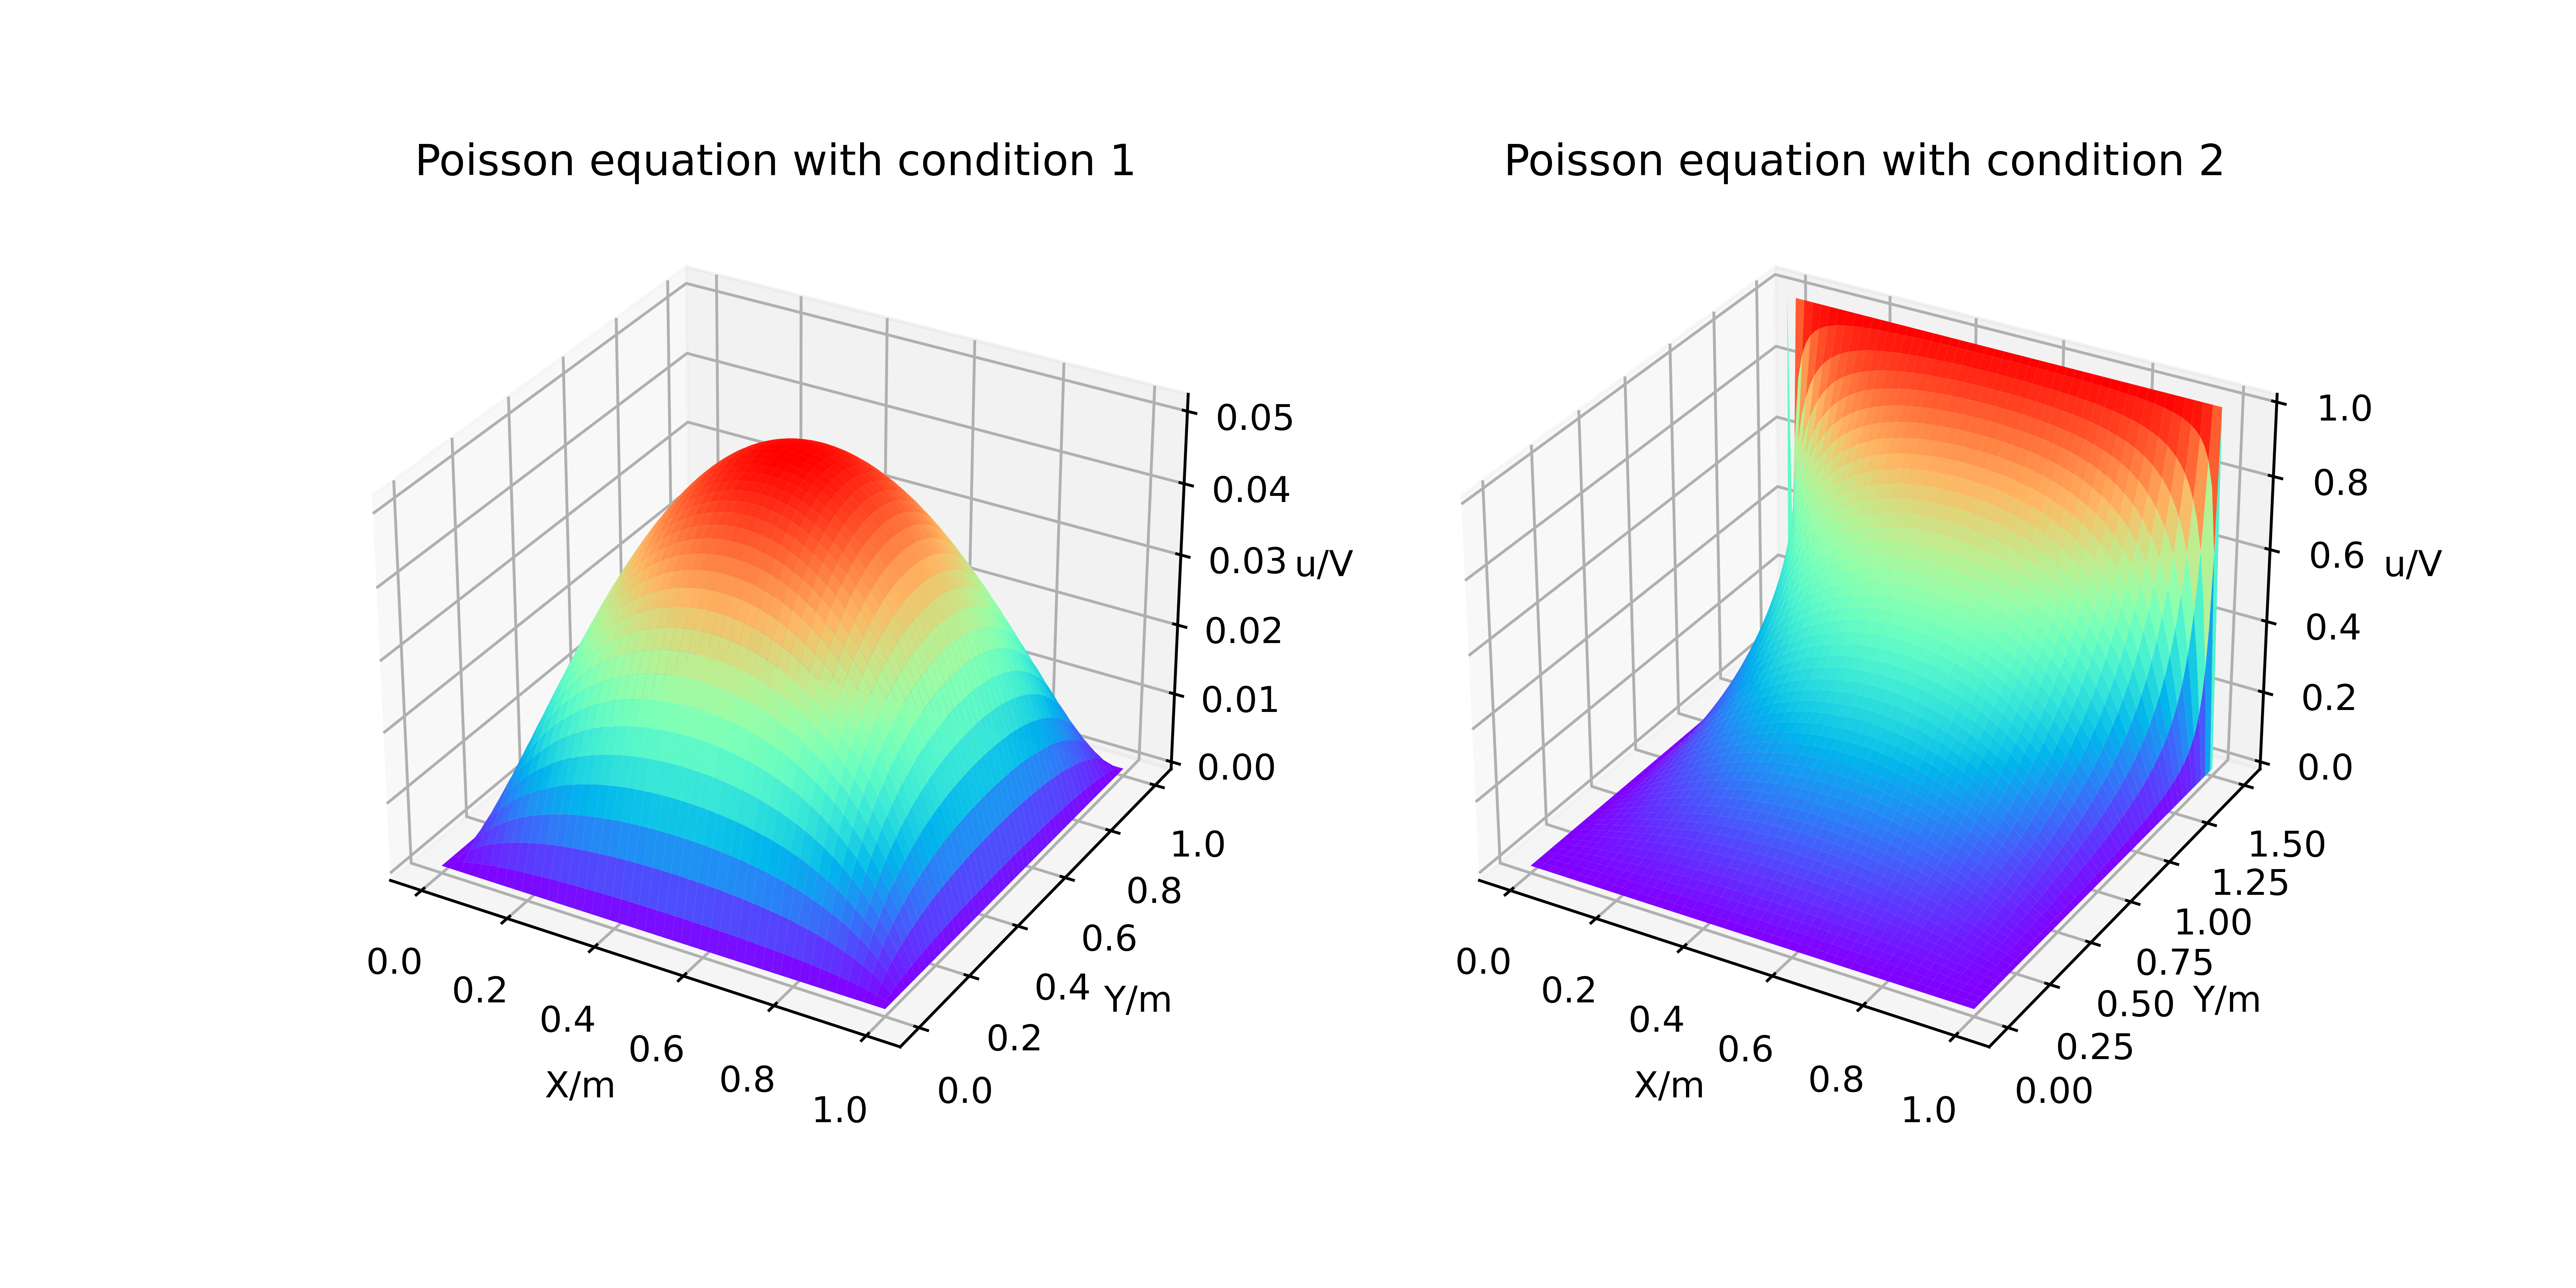
\includegraphics[width=1\linewidth]{photo/solvePoisson.png}
    \caption{泊松方程求解结果}
    \label{fig:1}
  \end{figure}

  \begin{figure}
    \centering
    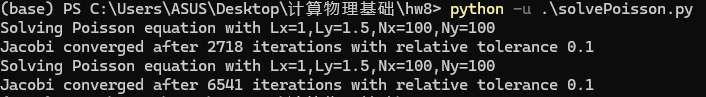
\includegraphics[width=0.6\linewidth]{photo/figp1.png}
    \caption{题目1程序运行截图}
    \label{fig:p1}
  \end{figure}

\section{题目2}
\subsection{题目描述}
Solve the time-dependent Schrödinger equation using both the Crank–Nicolson scheme and a stable explicit scheme. Consider the one-dimensional case and test it by applying it to the problem of a square well with a Gaussian initial state coming in from the left.

Hint: The Gaussian initial state could be expressed as:
\[
\Psi(x, 0) = \sqrt{\frac{1}{\pi}} \exp \left[ i k_0 x - \frac{(x - \xi_0)^2}{2} \right]
\]

\subsection{程序描述}
本程序将使用Crank-Nicolson方法和稳定的显式方法求解一维含时薛定谔方程。为简便,我们取$\hbar=m=1$
\[-\frac{1}{2} \frac{\partial^2 \Psi(x, t)}{\partial x^2} + V(x) \Psi(x, t)=i\frac{\partial \Psi(x, t)}{\partial t}
\]
其中
\[
V(x) =
\begin{cases}
0, & -a \leq x \leq a \\
V_0, & x < -a \text{ 或 } x > a
\end{cases}
\]
本题中我们取$a=2.0,V_0=-1.0,\xi_0=-5.0,k_0=1.0$,并取空间区间为$[-20,20]$,在边界处近似认为有边界条件$\Psi(-20)=\Psi(20)=0$。

  做离散化$(\frac{\partial^2 \Psi(x, t)}{\partial x^2})^n={\frac{\Psi_{i+1}^n-2\Psi_{i}^n+\Psi_{i-1}^n}{\Delta x^2}}$,$(\frac{\partial \Psi(x, t)}{\partial t})^n=\frac{\Psi_{i+1}^n-\Psi_i^n}{\Delta t}$

  考虑:
\[\theta (-\frac{1}{2} \frac{\partial^2 \Psi}{\partial x^2} + V \Psi)^n+(1-\theta)(-\frac{1}{2} \frac{\partial^2 \Psi}{\partial x^2} + V \Psi)^{n+1}=c\]

得到差分格式:
\[\Psi^{n+1}=(2iI-\theta V-\alpha \theta L)^{-1}(2iI+(1-\theta) V+(1-\theta) \alpha L)\Psi^{n}\]

其中$\alpha=\frac{\Delta t}{\Delta x^2},V_{ii}=V(x_i)$
\[
L=\begin{pmatrix}
2 & -1 & 0 & 0 & \cdots & 0 \\
-1 & 2 & -1 & 0 & \cdots & 0 \\
0 & -1 & 2 & -1 & \cdots & 0 \\
0 & 0 & -1 & 2 & \cdots & 0 \\
\vdots & \vdots & \vdots & \vdots & \ddots & \vdots \\
0 & 0 & 0 & 0 & \cdots & 2
\end{pmatrix}
\]
取$\theta=\frac{1}{2}$,为Crank–Nicolson格式,取$\theta=0$为Explicit格式。

若取$(\frac{\partial \Psi(x, t)}{\partial t})^n=\frac{\Psi_{i+1}^{n+1}-\Psi_i^{n-1}}{\Delta t}$,考虑:
\[(-\frac{1}{2} \frac{\partial^2 \Psi}{\partial x^2} + V \Psi)^n=(\frac{\partial \Psi(x, t)}{\partial t})^n\]
则得到Stable Explicit格式:
\[\Psi^n=\Psi^{n-1}-i \alpha L \psi^n-2i V dt\Psi^n\]

本程序源文件为solveSchrodinger.py,在终端进入当前目录,使用命令python -u solveSchrodinger.py运行本程序。使用python -u solveSchrodinger.py --test\_convergence SE或python -u solveSchrodinger.py --test\_convergence CN运行收敛性测试。运行时请保证Python第三方库Numpy,Matplotlib已安装。程序开发环境为Python3.12.3,可在Python3.8以上版本中运行。

\subsection{伪代码}
\subsubsection*{Crank–Nicolson和Stable Explicit格式求解伪代码}
\begin{breakablealgorithm}
  \caption{SchrodingerSolver}
  \begin{algorithmic}
  
  \State \textbf{Class} $SchrodingerSolver(Lx, Nx, V, dt)$ \Comment{Solve Schrodinger equation}
  \State $V, Lx, Nx, dx, dt, xl, u, Bmat, Vmat, Acn$ \Comment{Class attributes}
  
  \State \textbf{Method}
  \Function{initGrid}{}
    \State $xl \gets$ linspace($-Lx, Lx, Nx$)
    \State $u \gets$ zerosLike($xl$, dtype=complex)
    \State applyBoundary($u$)
  \EndFunction
  
  \Function{applyBoundary}{u}
    \State $u[0], u[-1] \gets 0.0 + 0.0j$
  \EndFunction
  
  \Function{setInitialCondition}{u0}
    \State $u \gets u0(xl)$
    \State applyBoundary($u$)
  \EndFunction
  
  \Function{updateU}{u}
    \State $u \gets u$
    \State applyBoundary($u$)
  \EndFunction
  
  \Function{initCrankNicolsonMat}{theta}
    \State \textbf{INPUT:} $theta$ (float, default $0.5$)
    \State $ap \gets \frac{dt}{dx^2}$
    \State $B \gets$ zeros($Nx, Nx$)
    \State $V \gets$ zeros($Nx, Nx$)
    \State $I \gets$ eye($Nx$)
    \For{$i \gets 0$ \To $Nx - 1$}
      \State $B[i, i] \gets 2$
      \State $V[i, i] \gets V(xl[i]) \cdot dt$
      \State \textbf{else for} $i < Nx - 1$
        \State $B[i, i+1] \gets -1$
        \State $B[i+1, i] \gets -1$
    \EndFor
    \State $A \gets$ inv($I \cdot 2j - 2 \cdot theta \cdot V - theta \cdot ap \cdot B$) @ \\
      \hspace{2em} ($I \cdot 2j + 2 \cdot (1 - theta) \cdot V + (1 - theta) \cdot ap \cdot B$)
    \State $Acn \gets A$
  \EndFunction
  
  \Function{crankNicolson}{maxStep}
    \State \textbf{INPUT:} $maxStep$ (integer, number of iterations)
    \State $ul \gets$ emptyList()
    \For{$i \gets 0$ \To $maxStep - 1$}
      \State $phi2 \gets$ abs($u$)$^2$
      \State append($ul, u$)
      \State updateU($Acn \cdot u$)
    \EndFor
    \State \Return array($ul$)
  \EndFunction
  
  \Function{stableExplicit}{maxStep}
    \State \textbf{INPUT:} $maxStep$ (integer, number of iterations)
    \State $ap \gets \frac{dt}{dx^2}$
    \State initCrankNicolsonMat($\theta=0.5$)
    \State $ul \gets$ [$u$]
    \State updateU($Acn \cdot u$)
    \State append($ul, u$)
    \For{$i \gets 0$ \To $maxStep - 1$}
      \State $phi2 \gets$ abs($u$)$^2$
      \State append($ul, u$)
      \State updateU($ul[-2] - 1j \cdot ap \cdot Bmat \cdot u - 2j \cdot dt \cdot Vmat \cdot u$)
    \EndFor
    \State \Return array($ul$)
  \EndFunction
  
  \end{algorithmic}
  \end{breakablealgorithm}

\subsection{输入输出实例}
本程序中使用python -u solveSchrodinger.py运行后将会生成图\ref{fig:4}至图\ref{fig:7}于当前目录下,分别为不同参数下($\alpha$从0.06到0.51),Crank–Nicolson,Stable Explicit,Explicit的求解结果。
程序运行截图如图\ref{fig:p2}所示。


\begin{figure}[h]
  \centering
  \includegraphics[width=1\linewidth]{photo/solveSchrodinger_Nx=100_dt=0.010.png}
  \caption{求解结果$\alpha=0.0613$}
  \label{fig:4}
\end{figure}


\begin{figure}[H]
  \centering
  \includegraphics[width=1.1\linewidth]{photo/solveSchrodinger_Nx=112_dt=0.010.png}
  \caption{求解结果$\alpha=0.0770$}
  \label{fig:5}
\end{figure}

\begin{figure}[H]
  \centering
  \includegraphics[width=1.1\linewidth]{photo/solveSchrodinger_Nx=283_dt=0.010.png}
  \caption{求解结果$\alpha=0.4970$}
  \label{fig:6}
\end{figure}

\begin{figure}[H]
  \centering
  \includegraphics[width=1.1\linewidth]{photo/solveSchrodinger_Nx=284_dt=0.010.png}
  \caption{求解结果$\alpha=0.5006$}
  \label{fig:7}
\end{figure}

\begin{figure}[H]
  \centering
  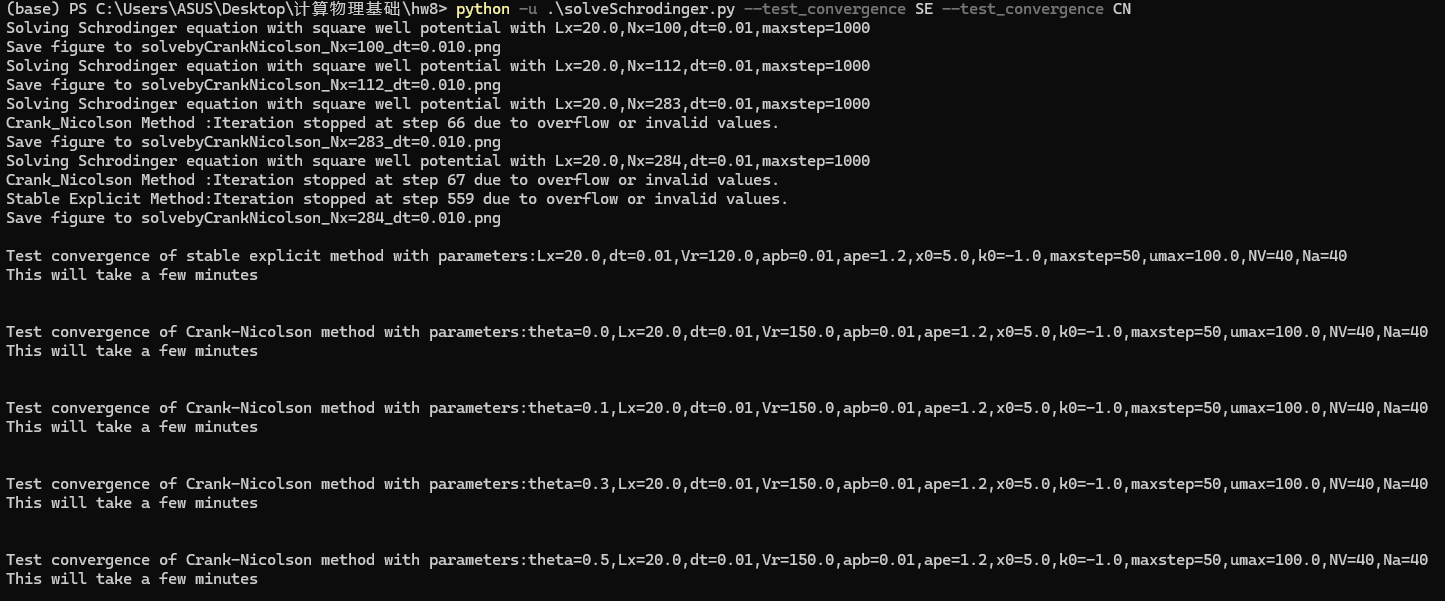
\includegraphics[width=0.8\linewidth]{photo/figp2.png}
  \caption{题目2程序运行截图}
  \label{fig:p2}
\end{figure}

\subsection{讨论}
根据图\ref{fig:4}至图\ref{fig:7},我们可以看到,Crank–Nicolson格式始终保持稳定,在大约$\alpha>0.0613$后,Explicit格式开始不稳定(图\ref{fig:4}-\ref{fig:5}),这说明对于普通的Explicit格式对于求解含时薛定谔方程并不适合。

另外我们注意到在$\alpha>0.5$后,Stable Explici格式也开始不稳定(\ref{fig:6}-\ref{fig:7})。这与PPT上给出的参考文献(J. Chem. Phys. 68, 2794 (1978)
)中的描述不符。其中作者宣称:"\textit{The stability of the proposed explicit scheme is seen to be governed by the same criterion as the Crank-NichOlson method.}"(图\ref{fig:p3})。我检查了其中对于稳定性的推导,发现其存在错误,正确过程如下:

采用von Neumann分析,令$\psi_j^n=\xi^n e^{i j K}$,带入差分格式得到:
\[\xi^2-2i(\alpha coskx -\alpha -V_j \Delta t)\xi=1=0\]
解为:
\[\xi_{1,2}=-i[\alpha coskx-\alpha -V_j \Delta t] \pm \sqrt{-(\alpha coskx-\alpha-V_j \Delta t)^2+1}\]
论文中认为$|\xi_{1,2}|=1$,因此该差分格式是恒稳定的。


但事实上,$|\xi_{1,2}|=1$要求第二项为实数,即$-(\alpha coskx-\alpha-V_j \Delta t)^2+1=1-\gamma^2<0>=0$。若
$1-\gamma^2<0$,则$\xi_{1,2}=-i(\gamma \pm \sqrt{\gamma^2-1})$,$\gamma$.这时$|\xi_2|=\gamma+ \sqrt{\gamma^2-1}>0$格式不稳定。

因此,Stable Explicit格式稳定的条件应是:
\[(\alpha coskx-\alpha-V_j \Delta t)^2<1 \quad for \quad any \quad V_j \quad and \quad kx\]

由于$\alpha>0,coskx \epsilon [-1,1]$,对有限方势阱:$V_j=V_0 or 0$,我们可以得到稳定的区域为由以下不等式围成的区域:
\[
\begin{cases} 
-1<2\alpha+V_0 dt<1, \\
-1<V_0 dt<1, \\
0<\alpha<1
\end{cases}
\]

我们改变$V_0$和$\alpha$测试在不同参数下求解的稳定性,得到稳定区域如图\ref{fig:8},可以看到其与上式给出的范围一致。

我们也测试了不同$\theta$下,类Crack-Nicolson格式的稳定性,得到不同$\theta$稳定区域如图\ref{fig:9}。可以看到随着$\theta$增大,稳定的参数区域逐渐增大,直到$\theta=0.5$时,对任何参数都稳定。



\begin{figure}[H]
  \centering
  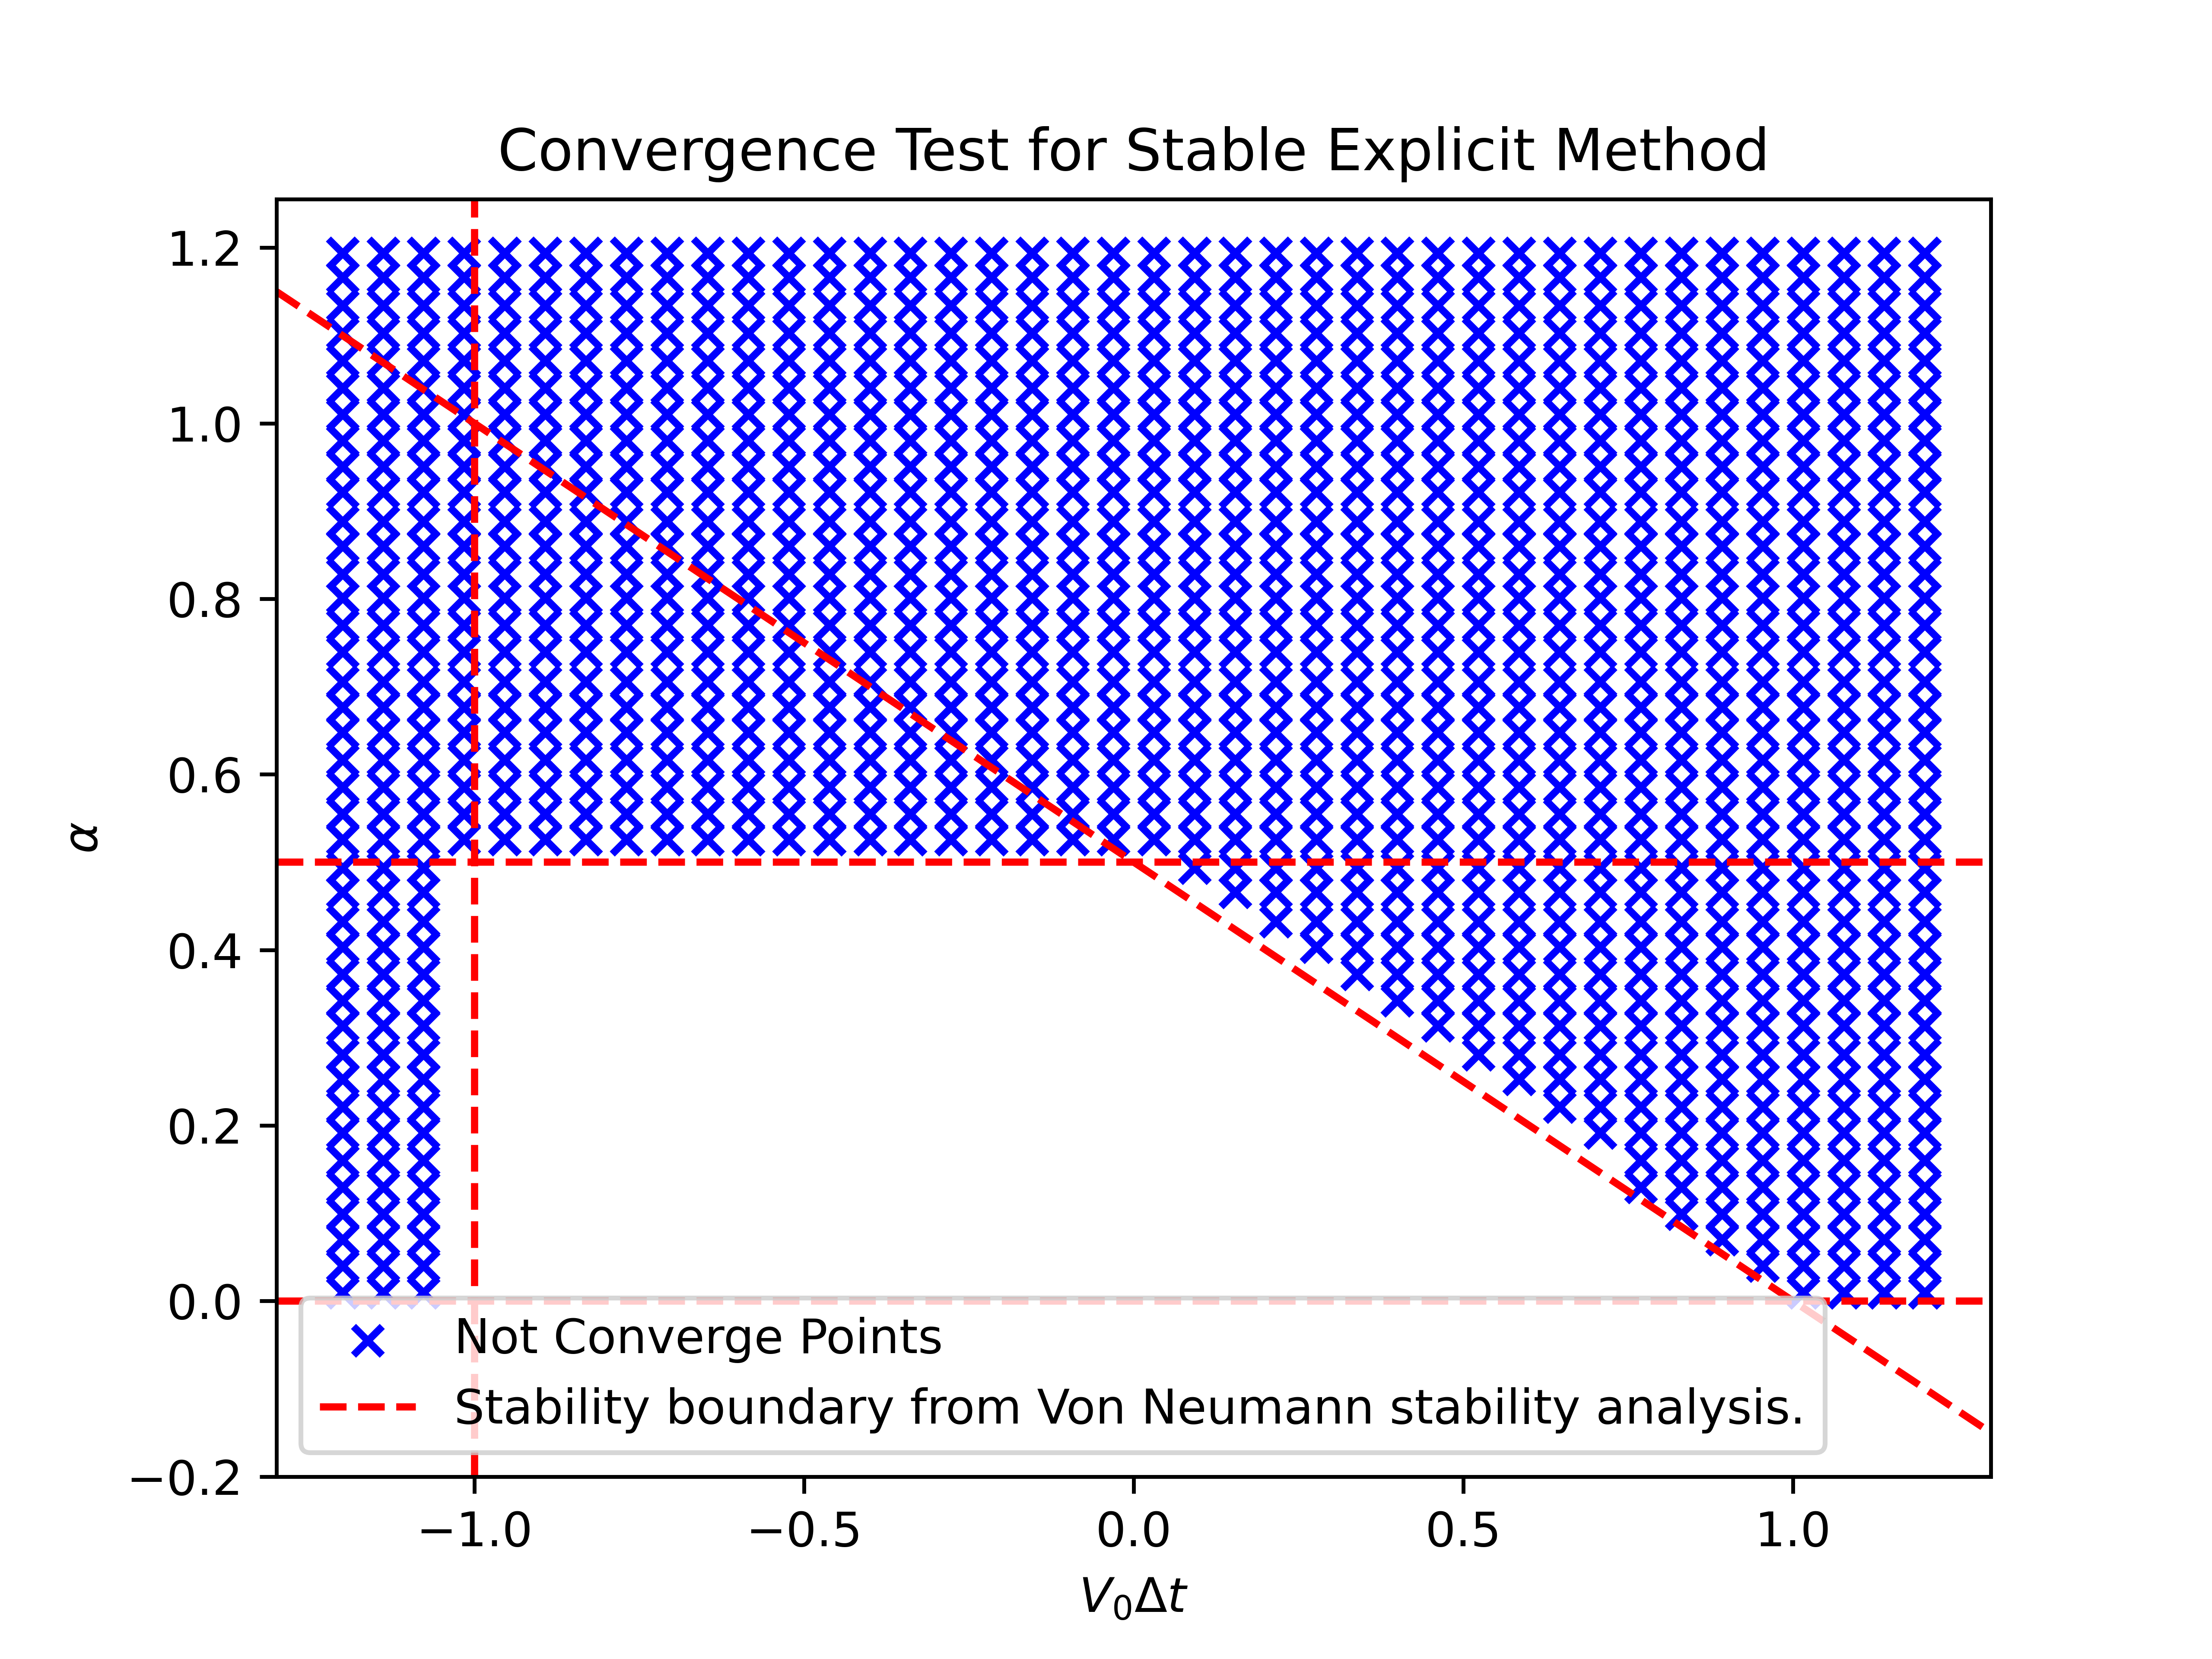
\includegraphics[width=0.8\linewidth]{photo/ConvergenceTestStableExplicit.png}
  \caption{不同$\alpha,V_0 \Delta t$Stable Explicit格式的稳定性}
  \label{fig:8}
\end{figure}


\begin{figure}[H]
  \centering
  \includegraphics[width=1\linewidth]{photo/ConvergenceTestCrankNicolson.png}
  \caption{不同$\theta,\alpha,V_0 \Delta t$类Crank Nicolson格式的稳定性}
  \label{fig:9}
\end{figure}

\begin{figure}[H]
  \centering
  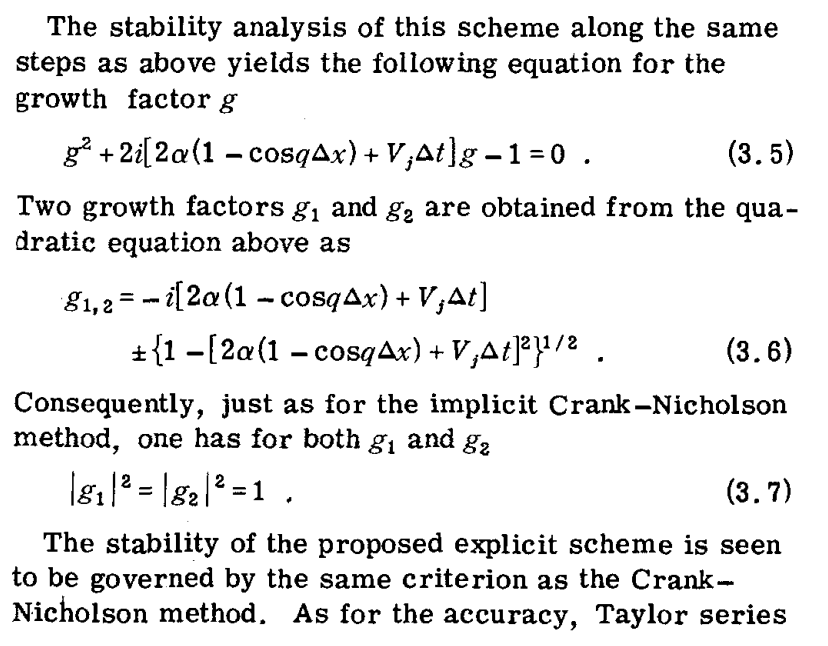
\includegraphics[width=0.8\linewidth]{photo/figp3.png}
  \caption{求解结果,$\alpha$}
  \label{fig:p3}
\end{figure}

\section{题目3}
\subsection{题目描述}
Prove the stability condition of the explicit scheme of the 1D wave equation by performing Von Neumann stability analysis:

\[
\frac{\partial^2 u}{\partial t^2} = c^2 \frac{\partial^2 u}{\partial x^2}.
\]

If \( \frac{c \Delta t}{\Delta x} \leq 1 \), the explicit scheme is stable.

\subsection{证明}
做离散化:
\[
\left(\frac{\partial^2 u(x, t)}{\partial x^2}\right)^n = \frac{u_{j+1}^n - 2u_j^n + u_{j-1}^n}{\Delta x^2},
\quad
\left(\frac{\partial^2 u(x, t)}{\partial t^2}\right)^n = \frac{u_j^{n+1} - 2u_j^n + u_j^{n-1}}{\Delta t^2}
\]

得到:
\[
u_j^{n+1} = 2u_j^n - u_j^{n-1} + \alpha^2 \left( u_{j+1}^n - 2u_j^n + u_{j-1}^n \right),
\]
其中,\(\alpha = \frac{c^2 \Delta t^2}{\Delta x^2}\)。


采用von Neumann分析,令$\psi_j^n=\xi^n e^{i j K}$,带入差分格式得到:
\[\xi^2-2 \beta  \xi +1=0,\beta=1+\alpha^2(coskx-1)\]
解为:$\xi_{1,2}=\beta \pm \sqrt{\beta^2-1}$

当$\beta>1$,$|\xi_2|=\beta+\sqrt{\beta^2-1}>1$,当$\beta<-1$,$|\xi_1|=-\beta+\sqrt{\beta^2-1}>1$,不稳定。当$\beta^2-1<0$,$|\xi_{1,2}|^2=1$,差分格式稳定。

因此要求$\beta=1+\alpha^2(coskx-1) \epsilon [-1,1]$。而$coskx \epsilon [-1,1]$,因此$\alpha^2 \epsilon [0,1]$,即$\frac{c \Delta t}{\Delta x} \leq 1$时,差分格式稳定。

\end{document}


